\chapter{Horarios}

\section{Acceso a los horarios}

Los horarios de los grados (\href{\linkCalendarGEI}{\acrshort{GEI}}, \href{\linkCalendarGCED}{\acrshort{GCED}} y \href{\linkCalendarGIA}{\acrshort{GIA}}) pueden encontrarse en sus correspondientes apartados de la página web de la \href{\linkFIC}{\acrshort{FIC}}. Los másteres suelen publicar sus horarios en sus respectivas páginas web.

\begin{curiosityBox}
    Los horarios de un curso son aprobados a finales del curso académico anterior, por lo que pueden ser consultados antes del comienzo de las clases.
\end{curiosityBox}


\section{Nomenclatura de los horarios}

Los horarios siguen la \textbf{nomenclatura}  ``\texttt{c.ACRONIMO.xy}", donde:
\begin{itemize}
    \item `\texttt{c}' es un valor numérico que indica el curso de la asignatura.
    
    \item `\texttt{ACRONIMO}' es un valor alfanumérico que corresponde al acrónimo, sigla o abreviatura de la asignatura.
    
    \item `\texttt{xy}' es el código del grupo y está compuesto por uno o dos dígitos.
\end{itemize}

Los \textbf{grupos de teoría} se identifican con \textbf{un único valor numérico} (\texttt{x}).

Los \textbf{grupos de prácticas} se identifican con \textbf{dos valores numéricos} (\texttt{xy}): el primero (\texttt{x}) corresponde al grupo de teoría del que deriva el grupo de prácticas, el segundo (\texttt{y}) identifica el propio subgrupo de prácticas.

\begin{exampleBox}
    \texttt{1.Cal.12} corresponde al grupo 2 de prácticas del grupo 1 de teoría de la asignatura de Cálculo en el primer curso.
\end{exampleBox}

\section{Asignación de los horarios del alumnado}

La \textbf{asignación de alumnos a grupos} la realiza el centro \textbf{antes del inicio de clases}. Este proceso se realiza de \textbf{forma secuencial} entre los estudiantes matriculados en un mismo estudio, siguiendo el \textbf{orden alfabético} de apellidos (comenzando según el \textbf{sorteo anual de letras de prioridad} en los procedimientos de admisión de la Xunta de Galicia) e intentando respetar, en la medida de lo posible, la \textbf{preferencia de franja horaria} (mañana o tarde) elegida por cada estudiante.

\begin{exampleBox}
    En el curso 2024/2025 las letra iniciales elegidas fueron `OA' para la prioridad del primer apellido.
\end{exampleBox}

\subsection{Selección de preferencia del horario}

La preferencia de franja horaria (mañana o tarde) puede indicarse en \href{\linkEspazosUDC}{Espazos UDC}. Primero debe seleccionarse el centro (Facultade de Informática) y luego acceder a la sección del menú ``\href{https://espazos.udc.es/centers/614/timetable/preference}{as miñas opcións/preferencia de horario de docencia}".

\FloatBarrier
\begin{figure}[htp]
    \centering
    \frame{
        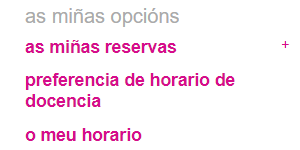
\includegraphics[width=0.3\linewidth]{figures/horarios/Horarios_Preferencia.png}
    }
\end{figure}
\FloatBarrier

Los horarios se generarán \textbf{automáticamente} teniendo en cuenta varios factores, principalmente: los \textbf{apellidos}, las \textbf{preferencias} (mañana o tarde), y las combinaciones de \textbf{asignaturas} en las que el alumnado esté matriculado y las \textbf{plazas} disponibles en los grupos docentes.

Para cada estudiante se buscará la mejor combinación de \textbf{horarios compatibles} entre todas las asignaturas de su matrícula, evitando solapamientos entre ellas, teniendo en cuenta preferencias y dando \textbf{prioridad a las asignaturas de los últimos cursos} en los que esté matriculado. La asignación dependerá de las plazas disponibles en los grupos docentes en el momento de realizar la asignación.

Para el alumnado que esté matriculado en \textbf{un solo curso}, el horario será \textbf{todo de mañana o todo de tarde}. Para el alumnado que esté matriculado en asignaturas de \textbf{más de un curso}, es probable que no sea posible ubicarlas todas en la misma franja horaria, aunque siempre se respetará la \textbf{misma franja horaria para las asignaturas de un mismo curso}.

\begin{warningBox}
    La selección de preferencia \textbf{no garantiza} una franja horaria en la franja elegida.
\end{warningBox}

\begin{warningBox}
    Algunos cursos (o estudios) no disponen de ambas franjas horarias.
\end{warningBox}

\begin{importantBox}
    En el caso de que no se pueda encontrar una solución, es posible que algunas de las asignaturas \textbf{se solapen}. Para solventar esto, será podrá solicitarse un \textbf{cambio de grupo}.
\end{importantBox}

\subsection{Visualización del horario asignado}

El resultado de la asignación de los grupos y horarios asignados puede consultarse en \href{\linkEspazosUDC}{Espazos UDC} en la sección del menú  ``\href{https://espazos.udc.es/centers/614/timetable/preference}{as miñas opcións/o meu horario}".

\begin{importantBox}
    Para cualquier \textbf{incidencia} (horario no asignado o asignatura no asignada en el horario), contactar con \href{mailto:vicedecanato.infrastruturas.fic@udc.gal}{\textbf{vicedecanato.infrastruturas.fic@udc.gal}} mediante correo electrónico.
\end{importantBox}

Los horarios son tablas con una \textbf{columna} para cada día de la semana de \textbf{lunes a viernes} y con una \textbf{fila} para cada \textbf{intervalo de 30 minutos}. Para cada \textbf{asignatura} se indica su \textbf{grupo} y el \textbf{aula o laboratorio} en la que se imparte.

\FloatBarrier
\begin{figure}[htp]
    \centering
    \frame{
        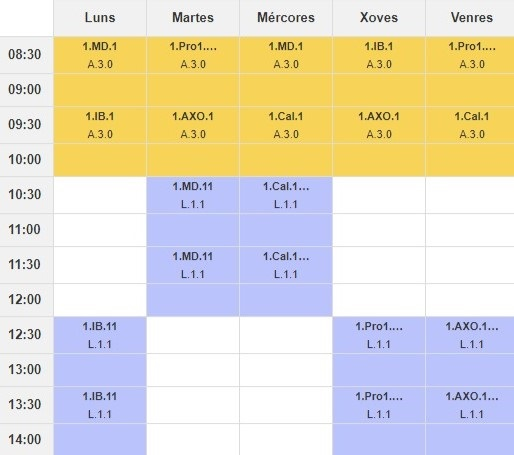
\includegraphics[width=0.5\linewidth]{figures/horarios/Horarios_Ejemplo.jpeg}}
\end{figure}
\FloatBarrier

\begin{infoBox}
    Las asignaturas de \textbf{color amarillo} (~\textcolor{colorTimetableTheory}{\fcolorbox{black}{colorTimetableTheory}{\rule{5pt}{5pt}}}~) corresponden a \textbf{clases de teoría} mientras que asignaturas de \textbf{color azul} (~\textcolor{colorTimetablePractice}{\fcolorbox{black}{colorTimetablePractice}{\rule{5pt}{5pt}}}~) corresponden a \textbf{clases de prácticas}.  
\end{infoBox}

\begin{curiosityBox}
    Los estudiantes de primera vez suelen estar asignados al mismo grupo de prácticas (y mismo grupo de teoría) en todas las materias que cursan.
\end{curiosityBox}

\subsection{Cambio de grupo}

Una vez realizada la asignación, es posible \textbf{cambiar de grupo docente} mediante dos procedimientos diferentes: la \textbf{permutación de grupos} y la \textbf{solicitud de cambio de grupo}.

% \subsubsection{Permutación de grupos}

La \textbf{permutación de grupos} consiste en el intercambio de común acuerdo entre estudiantes \textbf{con la misma matrícula} pero asignados a diferentes grupos.
Se realiza a través de un \textbf{formulario} que deberán cumplimentar recíprocamente los dos estudiantes implicados.

% \subsubsection{Solicitud de cambio de grupo}

La \textbf{solicitud de cambio de grupo} podrá utilizarse para solicitar cambios en sus horarios de forma justificada. Esta solicitud sólo se realizará cuando concurra alguna de las circunstancias enumeradas en la \href{https://www.fic.udc.es/sites/default/files/adjuntos_noticias/normativa_cambio_grupo_fic.pdf}{\textbf{normativa de cambio de grupo}}.

% \subsubsection{Plazos de cambio de grupo}

Los cambios de grupo se realizan en el mes de \textbf{septiembre}. Los plazos concretos se anuncian en la página web de la  \href{\linkFIC}{\acrshort{FIC}}.

\begin{exampleBox}
    A modo orientativo, los trámites de solicitud de intercambio y cambio de grupo del curso 2023/2024 comenzaron el 8 de septiembre. Los cambios aprobados entraron en vigor el 22 de septiembre.
\end{exampleBox}
